\documentclass[a4paper,1pt]{report}
\usepackage[utf8]{inputenc}
\usepackage[spanish]{babel}
\usepackage{amsfonts}
\usepackage{amsthm}
\usepackage{amssymb}
\usepackage{amsmath}
\usepackage{graphicx}
\usepackage{subcaption}
\usepackage{float}
\usepackage[rightcaption]{sidecap}

\newtheorem*{pbo}{Principio del Buen Ordenamiento}

\newtheorem*{pim}{Principio de Inducción Matemática}

\newtheorem*{teo}{Teorema}

\newtheorem*{cor}{Corolario}

\newtheorem*{dem}{Demostración}

\newtheorem*{dfn}{Definición}

\newtheorem*{lem}{Lema}

\newtheorem*{prp}{Propiedades}


% Title Page
\title{Conferencia 4 - Grafo Hamiltoniano}
\author{}

\begin{document}
\maketitle

\begin{dfn}[Camino Hamiltoniano o Cadena Hamiltoniana]
    Un camino $P = <v_1, v_2,..., v_k>$ es Hamiltoniano si $P$ es simple y contiene a todos los v\'ertices del grafo.
\end{dfn}

\begin{figure}[H]
    \centering
    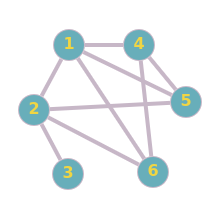
\includegraphics[width=0.2\textwidth]{figures4/G0.png}
    \caption{En el Grafo, el camino $<3,2,1,6,4,5>$ es Hamiltoniano.}
\end{figure} 



\begin{dfn}[Ciclo de Hamilton]
    Un ciclo $C = <v_1, v_2, ... v_k, v_1>$ en un grafo $G$ se dice de Hamilton (Hamiltoniano) si contiene a todos los v\'ertices del grafo.
\end{dfn}


\begin{figure}[H]
    \centering
    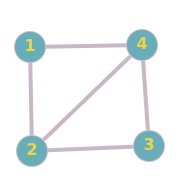
\includegraphics[width=0.2\textwidth]{figures4/SiHnoE.png}
    \caption{En el Grafo, el ciclo $<1,2,3,4,1>$ es Hamiltoniano.}
\end{figure} 

\begin{dfn}[Grafo Hamiltoniano]
    Un grafo conexo es Hamiltoniano si tiene un ciclo de Hamilton.
\end{dfn}


\textbf{Nota:} Aunque las definiciones de \textit{Grafo Euleriano} y \textit{Grafo Hamiltoniano} son similares (el primero busca recorrer todas las aristas del grafo sin repetirlas y el segundo recorrer todos los v\'ertices sin repetici\'on) no existe ninguna relaci\'on entre estas clasificaciones en un grafo. Es decir un grafo $G$ puede ser Hamiltoniano y no ser Euleriano y viceversa.

\begin{figure}[H]
    \centering
    \begin{subfigure}[b]{0.45\textwidth}
    \centering
    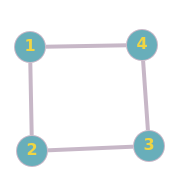
\includegraphics[width=0.4\textwidth]{figures4/C4.png}
    \caption{Grafo Hamiltoniano y Euleriano}
    \end{subfigure}
    \begin{subfigure}[b]{0.45\textwidth}
        \centering
    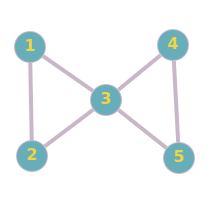
\includegraphics[width=0.4\textwidth]{figures4/noHsiE.png}
    \caption{Grafo Euleriano y no Hamiltoniano}
    \end{subfigure}
    \begin{subfigure}[b]{0.45\textwidth}
        \centering
    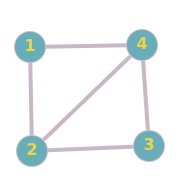
\includegraphics[width=0.4\textwidth]{figures4/SiHnoE.png}
    \caption{Grafo Hamiltoniano y no Euleriano}
    \end{subfigure}
    \begin{subfigure}[b]{0.45\textwidth}
    \centering
    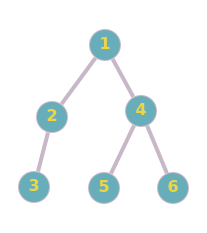
\includegraphics[width=0.4\textwidth]{figures4/arbol.png}
    \caption{Grafo ni Hamiltoniano ni Euleriano}
    \end{subfigure}
\end{figure} 


\begin{lem}
    Todo grafo completo G, $|V(G)|\geq 3$, es Hamiltoniano. 
\end{lem}
   
   
   \begin{dem}[Demostración por Inducción en $n = |V(G)|$]\end{dem}
   
   \textbf{Caso base}: Para $n=3$, $K_3$  tiene el ciclo  $<v_1,v_2,v_3,v_1>$ que es Hamiltoniano.
   
   \textbf{Hipótesis}: Supongamos que el grafo completo de $n$ v\'ertices ($K_n$) posee un ciclo de Hamilton.
   
   \textbf{Paso inductivo}: Sea $G$ un grafo completo de $n+1$ v\'ertices ($K_{n+1}$), si construimos $G' = G - v$ (le quitamos un v\'ertice a G), el grafo $G'$ es $K_n$, es decir es un grafo completo de $n$ v\'ertices.
   En $G'$ se cumple la hip\'otesis de inducci\'on, luego en $G'$ hay un ciclo de Hamilton.   
   Sea el ciclo Hamiltoniano $C = <v_1,v_2,\dots,v_n,v_1>$ de $G'$, entonces si se añade nuevamente el vértice $v$ y todas sus aristas se vuleve a obtener $K_{n+1}$ y como $v$ est\'a enlazado a todos los dem\'as v\'ertices, sabemos que las aristas $\{v, v_n\}$ y $\{v, v_1\} \in E(G)$, entonces se puede tener el ciclo $C' = <v_1,v_2,\dots,v_n,v,v_1>$ que es un ciclo Hamiltoniano en $K_{n+1}$ $\blacksquare$. 
   
   \begin{teo}
    Si un grafo G es Hamiltoniano entonces para cualquier subconjunto no vacío de vértices S de G, el número de componentes conexas del subgrafo $G - S$ es menor o igual que  $|S|$.
   \end{teo}

   \begin{dem}[Demostración del Teorema]\end{dem}

    Como $G$ es Hamiltoniano, tiene un ciclo que es de Hamilton.  
    Cuando se remueven los vértices del conjunto $S$ de $G$, el ciclo Hamiltoniano se divide en a lo sumo $|S|$ segmentos~(cadenas de vértices consecutivos del ciclo que no contienen vértices de S). 
    Cada segmento corresponde a una componente conexa de $G-S$ si no existen aristas adicionales en G que estén fuera del ciclo y que conecten a estos segmentos. Si existieran estas aristas, entonces conectarían segmentos y, con ello, se reduciría el número de componentes conexas. 
    Luego, el número de componente conexas del subgrafo $G - S$ es menor o igual que  $|S|$ $\blacksquare$.
   


\begin{dfn}[Clausura de un Grafo]
    Dado un grafo $G$ con $|V(G)| = n$, se define inductivamente la secuencia de grafos $G_0, G_1,..., G_k$, donde $G_0 = G$ y $G_{i+1} = G_i + \{u,v\}$, donde $u,v$ son v\'ertices no adyacentes de $G_i$ tales que $deg_{G_i}(v) + deg_{G_i}(u) \geq n$. Tras aplicar este procedimiento, el \'ultimo grafo que se ontiene es la clausura de $G$ y se denota $clausura(G)$ 
\end{dfn}


\begin{figure}[H]
    \centering
    \begin{subfigure}[b]{0.3\textwidth}
    \centering
    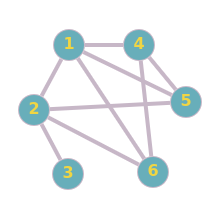
\includegraphics[width=0.5\textwidth]{figures4/G0.png}
    \caption{$G_0 = G$}
    \end{subfigure}
    \begin{subfigure}[b]{0.3\textwidth}
        \centering
    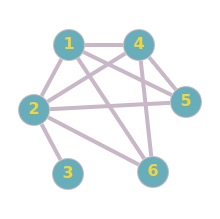
\includegraphics[width=0.5\textwidth]{figures4/G1.png}
    \caption{$G_1 = G_0 + \{2,4\}$}
    \end{subfigure}
    \begin{subfigure}[b]{0.3\textwidth}
        \centering
    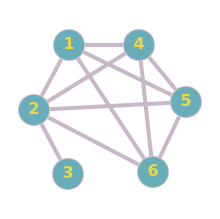
\includegraphics[width=0.5\textwidth]{figures4/G2.png}
    \caption{$G_2 = G_1 + \{5,6\}$}
    \end{subfigure}
    \caption{Ejemplo del proceso de obtenci\'on de la clausura, en el ejemplo en grafo $G_2$ es la $clausura(G)$}
\end{figure} 

\begin{teo}
La operaci\'on de clausura de un grafo, es una operaci\'on bien definida. (Sin importar el orden en que se adicionen las aristas durante la construcci\'on de los $G_i$ intermedios, el grafo final, que es la clausura de $G$ es siempre el mismo)
\end{teo}

\begin{dem}[Reducci\'on al absurdo]\end{dem}
Sean $E = \{e_1,e_2, ... e_p\}$ y $F = \{f_1,f_2,..., f_r\}$, dos formas de construir la clausura de un grafo $G$. Es decir, la primera es $G_0 = G$, $G_1 = G + e_1$, $G_2 = G_1 + e_2$,..., $clausura_E(G) = G_{p-1} + e_{p}$; y la otra forma se\'ria $G_0 = G$, $G_1 = G_0 + f_1$, $G_2 = G_1 + f_2$,..., $clausura_F(G) = G_{r-1} + f_r$.
Para demostrar que $clausura_E(G) = clausura_F(G)$, basta con demostrar que $E = F$, para esto demostremos que $E \subseteq F$ y $F \subseteq E$. 

Para demostrar que $E \subseteq F$ hagamos una reducci\'on al absurdo, supongamos que esto no se cumple, entonces existen aristas en $E$ que no pertenecen al conjunto $F$. Tomemos del conjunto $E/F$ (que asumimos no vac\'io) la arista con menor \'indice, sea esta $e_i$. Como $e_i$ se agrega a la clausura uniendo los v\'ertices no adyacentes $u,v$ donde $deg_{G_{i-1}}(v) + deg_{G_{i-1}}(u) \geq n$. 
De donde $$deg_{G_{i-1}}(v) = deg_{G}(v) + X_v $$ con $X_v \geq 0$ siendo la cantidad de aristas en el conjunto $\{e_1, ...e_{i-1}\}$ que inciden en $v$, an\'alogamente 

$$deg_{G_{i-1}}(u) = deg_{G}(u) + X_u $$

Como todos los $e_j, 1\leq j \leq i-1$ pertenecen a $F$ entonces el conjunto $F = \{e_1, ..., e_{i-1} \} \cup \{f_1,f_2,..., f_r\}/\{e_1, ..., e_{i-1} \}$, de donde en la clausura construida por las aristas de conjunto $F$ se tiene que:

$$deg_{clausura_F}(v) = deg_G(v) +  X_v + Y_v$$

con $Y_v \geq 0$ cantidad de aristas del conjunto $\{f_1,f_2,..., f_r\}/\{e_1, ..., e_{i-1} \}$ que inciden en $v$, analogamente para $u$:


$$deg_{clausura_F}(u) = deg_G(u) +  X_u + Y_u$$

con $Y_u \geq 0$ cantidad de aristas del conjunto $\{f_1,f_2,..., f_r\}/\{e_1, ..., e_{i-1} \}$ que inciden en $u$, de donde:

$$deg_{clausura_F}(v) + deg_{clausura_F}(u) = deg_G(v) +  X_v + Y_v + deg_G(u) +  X_u + Y_u \geq $$
$$\geq deg_{G_{i-1}}(v) + deg_{G_{i-1}}(u) \geq n $$

Por tanto la arista $\{u, v\}$ se puede agregar a la $clausura_F$, resultando en una iteraci\'on m\'as en el algoritmo de obtenci\'on de la clausura, pero esto es una contradicci\'on ya que el grafo $clausura_F(G)$ tiene que ser el \'ultimo que se obtenga, de donde lo supuesto es falso y todas las aristas de $E$ pertenecen a $F$, es decir $E \subseteq F$.

La demostraci\'on de $F \subseteq E$ es an\'aloga a esta, por tanto $E = F$ y $clausura_E(G) = clausura_F(G)$.

La clausura es una operaci\'on bien definida $\blacksquare$.

\begin{teo}[Bondy-Chvátal]
    Sea $G$ un grafo donde $|V(G)|\geq 3$, $G$ es Hamiltoniano $\Leftrightarrow clausura(G)$ es Hamiltoniano.
\end{teo}

Demostrar este teorema es equivalente a demostrar que: $G_i$ es Hamiltoniano $\Leftrightarrow G_{i +1}$ es Hamiltoniano. Si se demuestra esto, entonces siguiendo la cadena de transitividad queda demostrado que: $G$ es Hamiltoniano $\Leftrightarrow clausura(G)$ es Hamiltoniano.
\begin{dem}[$\Rightarrow$] Si $G_i$ es Hamiltoniano entonces $G_{i +1}$ es Hamiltoniano\end{dem}

Como $G_i$ es Hamiltoniano, entonces posee un ciclo de Hamilton. 
Sea $C =  <v_1, v_2,..., v_k, v_1>$ el ciclo de Hamilton de $G_i$, este ciclo tambi\'en est\'a presente en $G_{i+1}$, porque $G_{i+1}$ no es m\'as que $G_i$ con una arista agregada. Luego $G_{i+1}$ es Hamiltoniano.

\begin{dem}[$\Leftarrow$] Si $G_{i+1}$ Hamiltoniano $\Rightarrow G_i$ Hamiltoniano \end{dem}

Sabemos que $G_{i+1} = G_{i} + \{x,y\}$ donde $x,y$ son v\'ertices no adyacentes en $G_i$ tales que $deg_{G_i}(x) + deg_{G_i}(y) \geq n$.

Como $G_{i+1}$ es Hamiltomiano, si el ciclo Hamiltoniano de $G_{i+1}$  no contiene a la arista $\{x,y\}$ (la agregada que no estaba en $G_i$), entonces este ciclo también aparecía en $G_i$, de donde $G_i$ Hamiltoniano.

Si $\{x,y\}$ s\'i aparece en el ciclo, en el grafo $G_i$, como no está $\{x,y\}$, pero si las restantes aristas, habrá un camino Hamiltoniano: 

$C=<v_0,v_1,\dots,v_{n-1}>$ donde $v_0=x$ y $v_{n-1}=y$.

Construyamos entonces un ciclo Hamiltoniano que no utilice la arista $\{x,y\}$, n\'otese que en la cadena $C$, tiene que existir alg\'un v\'ertice $v_j$ tal que $v_j$ sea adyacente a $x$ y $v_{j-1}$ sea adyacente a $y$.

\begin{figure}[H]
    \centering
    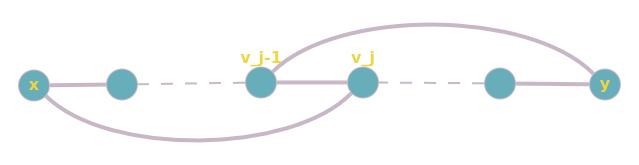
\includegraphics[width=0.5\textwidth]{figures4/clausura_demo.png}
\end{figure} 

Supongamos que esto no ocurra, entonces por cada adyacente a $x$ en la cadena, el v\'ertice anterior a este no puede ser adyacente a $y$, como la cadena es Hamiltoniana, contiene a todos los adyacentes de $x$, de donde $deg(y) \leq n - 1 - deg(x)$, de donde $deg(y) + deg(x) \leq n -1$, pero sabemos que esto no es posible, puesto que la arista $\{x,y\}$ se agrega a la clausura en el grafo $G_{i+1}$ y esto solo se hace si los v\'ertices no adyacentes $x,y$ complen que $deg(x) + deg(y) \geq n$.

Entonces lo supuesto es falso, por tanto existe $v_{j}$ en C tal que $v_j$ es adyacente a $x$, y $v_{j-1}$ es adyacente a $y$. 

Por tanto se puede tomar el ciclo $<v_0=x,v_{j},\dots,v_{n-1}=y,v_{j -1},v_{j-2},\dots,v_1,v_0=x>$ que es un ciclo Hamiltoniano.\\

Luego G es Hamiltoniano si y solo si su clausura lo es $\blacksquare$.

\begin{teo}[Dirac]
    Sea $G$ un grafo donde $|V(G)|= n\geq 3$, si $\forall v~ deg(v) \geq \frac{n}{2} ~ \Rightarrow G$ es Hamiltoniano 
\end{teo}

\begin{teo}[Ore]
    Sea $G$ un grafo donde $|V(G)|= n\geq 3$, si $\forall u,v$ no adyacentes $~ deg(u) + deg(v) \geq n ~ \Rightarrow G$ es Hamiltoniano 
\end{teo}

\begin{dem}[Directa]\end{dem}

N\'otese que el cumplimiento del \textit{Teorema de Ore} implica el cumplimiento del \textit{Teorema de Dirac}. 
Si en un grafo todos los v\'ertices tienen grado mayor o igual a $\frac{n}{2}$, entonces para cualquier pareja de v\'ertices no adyacentes $u, v$, $deg(u) + deg(v) \geq \frac{n}{2} + \frac{n}{2} = n$, donde el grafo cumple la hip\'otesis de \textit{Ore}.

Luego basta con demostrar el \textit{Teorema de Ore}. Como en $G$ todos los v\'ertices $u,v$ no adyacentes cumplen que $deg(u) + deg(v) \geq n$ entonces la $clausura(G) = K_n$, que sabemos tiene un ciclo de Hamilton, luego por el \textbf{Teorema de Bondy-Chvátal}, $G$ es Hamiltoniano.

\textbf{Nota:} Ambos teoremas son condiciones suficientes pero no necesarias, un grafo puede ser Hamiltoniano sin que sus v\'ertices cumplan esta condici\'on, por ejemplo:

\begin{figure}[H]
    \centering
    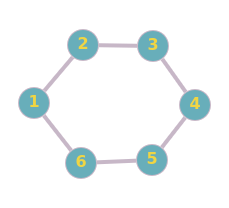
\includegraphics[width=0.2\textwidth]{figures4/C6.png}
    \caption{$C_6$ es Hamiltoniano y sin embargo todos sus v\'ertices son de grado $2$, por lo que la suma de los no adyacentes es $4 < 6$.}
\end{figure} 

\begin{cor}[Corolario del \textbf{Teorema de Ore}]
    Si $G$ es un grafo conexo, n vértices, con $n\geq 3$, en el cual $deg(u)+deg(v)\geq n - 1$ para todo par de vértices no adyacentes u, v, entonces $G$ posee un camino Hamiltoniano.
  \end{cor}
  
  \begin{dem}[Demostración del Corolario del \textbf{Teorema de Ore}]\end{dem}
  
  Sabemos que G es conexo, y con n vértices.
  Creamos el grafo $G' = G + w$, a partir de añadir el vértice $w$ y este lo conectamos con todos los vértices existentes.
  En $G'$ se cumpliría que $$deg(u)+deg(v)\geq n - 1 + 2 = n + 1$$ para todo par de vértices u, v no adyacentes,
  luego $G'$ es Hamiltoniano por el \textbf{Teorema de Ore}.
  
  Entonces existe un ciclo Hamiltoniano en $G'$ y este tiene que pasar por el vértice $w$. Entonces basta con eliminar este vértice y se tendría para G un camino Hamiltoniano $\blacksquare$.
  
\end{document} 